\documentclass[tikz,border=10pt]{standalone}
\usepackage{pgfplots}
\usetikzlibrary{arrows.meta, positioning, calc}

\begin{document}
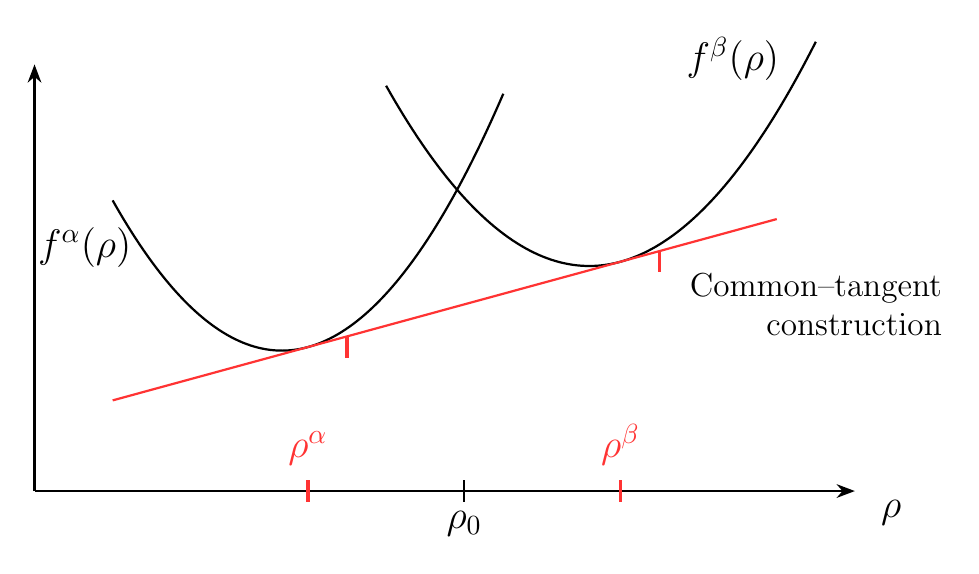
\begin{tikzpicture}
    \begin{axis}[
        % --- Axis Setup ---
        axis lines = left,
        xlabel = {$\rho$},
        ylabel = {},
        xlabel style = {at={(ticklabel* cs:1.02)}, anchor=north west, font=\Large},
        ylabel style = {at={(ticklabel* cs:1.02)}, anchor=south east},
        axis line style = {-Stealth, thick},
        ticks = none,
        % Domain and Range
        xmin = -0.5, xmax = 10,
        ymin = 0, ymax = 8,
        clip = false,
        width = 12cm,
        height = 7cm
    ]

        % --- Math Definitions ---
        \def\m{0.4}
        \def\c{1.5}
        \def\xa{3.0} % rho_alpha
        \def\xb{7.0} % rho_beta
        \def\kOne{0.6}
        \def\kTwo{0.5}

        % --- 1. The Curves ---

        % Curve Alpha (Left)
        \addplot[thick, black, domain=0.5:5.5, samples=100] 
            {\kOne*(x - \xa)^2 + \m*x + \c} 
            node[pos=0.1, anchor=east, font=\Large] {$f^\alpha(\rho)$};

        % Curve Beta (Right)
        \addplot[thick, black, domain=4.0:9.5, samples=100] 
            {\kTwo*(x - \xb)^2 + \m*x + \c}
            node[pos=0.9, anchor=south east, font=\Large] {$f^\beta(\rho)$};

        % --- 2. The Common Tangent (Red Line) ---
        \addplot[thick, red!80, domain=0.5:9] {\m*x + \c};

        % --- 3. Custom Ticks and Labels ---

        % Point rho_alpha
        \coordinate (P_alpha) at (axis cs:\xa, {\m*\xa + \c});
        \draw[very thick, red!80] ($(P_alpha)+(0,0.2)$) -- ($(P_alpha)+(0,-0.2)$);
        \draw[very thick, red!80] (axis cs:\xa, 0.2) -- (axis cs:\xa, -0.2);
        \node[red!80, font=\Large, anchor=south] at (axis cs:\xa, 0.3) {$\rho^\alpha$};

        % Point rho_beta
        \coordinate (P_beta) at (axis cs:\xb, {\m*\xb + \c});
        \draw[very thick, red!80] ($(P_beta)+(0,0.2)$) -- ($(P_beta)+(0,-0.2)$);
        \draw[very thick, red!80] (axis cs:\xb, 0.2) -- (axis cs:\xb, -0.2);
        \node[red!80, font=\Large, anchor=south] at (axis cs:\xb, 0.3) {$\rho^\beta$};

        % Point rho_0 (Middle)
        \def\xzero{5.0}
        \draw[thick, black] (axis cs:\xzero, 0.2) -- (axis cs:\xzero, -0.2);
        \node[black, font=\Large, anchor=north] at (axis cs:\xzero, -0.2) {$\rho_0$};

        % --- 4. Annotation Text (Updated to 2 lines) ---
        \node[align=right, font=\large] at (axis cs: 9.5, 3.5) {
            Common--tangent \\
            construction
        };

    \end{axis}
\end{tikzpicture}
\end{document}